      
               
                \begin{ledgroupsized}[r]{120mm}
                \footnotesize 
                \pstart                
                \noindent\textbf{\"{U}berlieferung:}   
                \pend
                \end{ledgroupsized}
            
              
                            \begin{ledgroupsized}[r]{114mm}
                            \footnotesize 
                            \pstart \parindent -6mm
                            \makebox[6mm][l]{\textit{L}}Konzept: LH XXXVII 2 Bl. 97. 1 Bl. 2\textsuperscript{o}. 2 S. zweispaltig. Linke Spalte fort\-laufender Text, rechte Spalte Korrekturen und Erg\"{a}nzungen. Auf Bl. 97 r\textsuperscript{o} obere H\"{a}lfte rechts die Zeichnung \textit{[Fig. 1]}. Geringe Textverluste am linken Seitenrand durch abgerissenes Papier.\\Cc 2, Nr. 492 A \pend
                            \end{ledgroupsized}
                \vspace*{8mm}
                \pstart 
                \normalsize
            \centering[97 r\textsuperscript{o}] Demonstratio \edtext{Nova}{\lemma{}\Afootnote{Nova \textit{ erg.} \textit{ L}}} Legum Refractionis\protect\index{Sachverzeichnis}{lex!refractionis},\\ quae in Lumine \edlabel{observanturstart}\edtext{observantur}{{\xxref{observanturstart}{observanturend}}\lemma{observantur}\Afootnote{ \textit{ (1) }\ Observatum dudum est Radium Lucis\protect\index{Sachverzeichnis}{radius!lucis|textit} ex \textit{(a)}\ aere transeuntem \textit{(b)}\ vitro  \textit{(aa)}\ in aerem transeuntem; \textit{(bb)}\ exeuntem, vel ex aere vitrum intrantem a cursu suo ita deflectere, ut sinus anguli quem facit ad \textit{ (2) }\  Mirum [...] perpendiculari. \textit{ L}}} \pend\vspace{1.0ex} \pstart Mirum semper omnibus visum est, Radios Lucis ex corpore raro in densius intrantes refringi ad perpendicularem, contra ex denso in rarum exeuntes refringi a perpendiculari\edlabel{observanturend}. \hspace{1mm}Contrarium \hspace{1mm}enim \hspace{1mm}evenire \hspace{1mm}debere \hspace{1mm}videbatur, quia \hspace{1mm}\edtext{radius}{\lemma{quia}\Afootnote{ \textit{ (1) }\ quod \textit{ (2) }\ radius \textit{ L}}} ad \pend \pstart \noindent perpendicularem refractus \edtext{medium}{\lemma{refractus}\Afootnote{ \textit{ (1) }\ ipsum corp \textit{ (2) }\ medium \textit{ L}}} citius fortiusque penetrat \edtext{ac profundius \edlabel{intratstart}intrat:}{\lemma{}\Afootnote{ac profundius intrat \textit{ erg.} \textit{ L}}} \edtext{at medium densius ab eadem vi tardius debiliusque penetrari debere\edlabel{intratend}}{{\xxref{intratstart}{intratend}}\lemma{intrat:}\Afootnote{ \textit{ (1) }\ jam medium quanto densius est, tanto tardius debiliusque ab eadem vi  \textbar\ quam \textit{ erg.}\ \textbar\  penetrari debere \textit{ (2) }\ at [...] debere \textit{ L}}}\edtext{}{\lemma{}\Afootnote{debere  \textbar\ videri poterat \textit{ gestr.}\ \textbar\ , ac \textit{ L}}}, ac radium\protect\index{Sachverzeichnis}{radius} proinde versus superficiem potius repelli, quam versus fundum refringi rationis erat. \edtext{Quemadmodum si supponatur superficies aquae vel Hydrargyri esse \textit{ab} baculus ligneus \textit{cd} versatilis circa \textit{c} patet}{\lemma{erat.}\Afootnote{ \textit{ (1) }\ Quemadmodum Mercurius\protect\index{Sachverzeichnis}{mercurius|textit} eundem baculum eadem vi impactum,  \textit{(a)}\ magis versus \textit{(b)}\ citiusque versus superficiem \textit{(c)}\ et in summo a manu   \textbar\ aliove obstaculo \textit{ erg.}\ \textbar\  retentum \textit{(aa)}\ magis \textit{(bb)}\ fortius citiusque versus superficiem inclinabit, quam aqua faceret. Esto in figura prima superficies liquoris (sive aquae sive Mercurii\protect\index{Sachverzeichnis}{mercurius!|textit}) \textit{ab} baculus liquorem intrans \textit{cd}  \textit{(aaa)}\  firmatus in \textit{c} \textit{(bbb)}\ versatilis circa \textit{c} appensumque ei in   \textbar\ altera \textit{ erg.}\ \textbar\  extremitate   \textbar\ \textit{d} \textit{ erg.}\ \textbar\  pondus. \textit{ (2) }\ Quemadmodum Mercurius\protect\index{Sachverzeichnis}{mercurius|textit} eundem baculum eadem vi impactum et a manu aliove obstaculo in summo ita petent. \textit{ (3) }\ Ut si \textit{ (4) }\ Quemadmodum si supponatur superficies  \textit{(a)}\ liquoris \textit{(b)}\ aquae [...] baculus  \textbar\ ligneus \textit{ erg.}\ \textbar\  \textit{cd} versatilis circa \textit{c} patet \textit{ L}}} facilius $\langle$i$\rangle$n aqua quam Hydrargyro\protect\index{Sachverzeichnis}{hydrargyrus} baculum ex \textit{cdd} in \textit{cd} depelli, aut ibi sustineri posse. \pend \vspace{1.0ex}
               %\begin{wrapfigure}{l}{0.6\textwidth}                    
               \begin{center}
               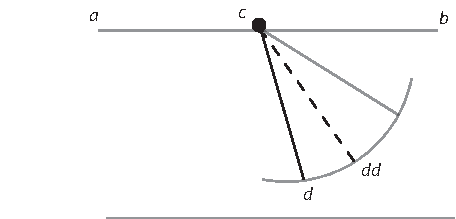
\includegraphics[width=0.6\textwidth]{images/37_2_97r}
               \\\hspace{15mm}\textit{[Fig. 1, tlw. Blindzeichnung]}
               %\end{wrapfigure}
               \end{center}
            \pstart Sed habet hoc natura $\langle$u$\rangle$t peculiares quasdam suas rationes secuta, saepe alia omnia $\langle$co$\rangle$gat, quam nos expectassemus.\pend \pstart Cartesius\protect\index{Namensregister}{\textso{Descartes} (Cartesius, des Cartes, Cartes.), Ren\'{e} 1596\textendash 1650} cum \edtext{agnovisset rationi experientiaeque consentaneum esse}{\lemma{cum}\Afootnote{ \textit{ (1) }\ recte demonstrasset corpus \textit{ (2) }\ agnovisset  \textit{(a)}\ Leges\protect\index{Sachverzeichnis}{lex!refractionis|textit} refractionis contrarias esse in corporibus tum \textit{(b)}\ rationi experientiaeque consentaneum esse \textit{ L}}}, ut corpus durum incidens ex liquido rariore in liquidum densius, refringatur \edtext{a}{\lemma{refringatur}\Afootnote{ \textit{ (1) }\ ad \textit{ (2) }\ a \textit{ L}}} perpendiculari, Lumen\protect\index{Sachverzeichnis}{lumen} tamen excepit a regula universali; corpora enim rariora luminis\protect\index{Sachverzeichnis}{lumen} respectu esse velut villosa, contra densiora esse quoque glabriora \edtext{supponit}{\lemma{}\Afootnote{supponit \textit{ erg.} \textit{ L}}}. Jam experientia constare corpus aliquod durum facilius corpus glabrum\hspace{1pt} quam\hspace{1pt} villo-\pend\pstart\noindent sum transire. \edtext{Ita}{\lemma{transire.}\Afootnote{ \textit{ (1) }\ Quemadmodum \textit{ (2) }\ Ita \textit{ L}}} enim globulum facilius in polito marmore quam tapete rugoso procurrere videmus.\edtext{}{\lemma{videmus.}\Bfootnote{\textsc{R. Descartes, }\cite{00038}\textit{La dioptrique}, Leiden 1637, S. 23 (\textit{DO} VI, S. 103). }}\pend \pstart Sed haec explicandi phaenomeni ratio, paucissimis, si in verba Magistri jurare paratos excipias, \edlabel{satisfecitstart}\edtext{satisfecit.}{{\xxref{satisfecitstart}{satisfecitend}}\lemma{satisfecit.}\Afootnote{ \textit{ (1) }\ Praeterquam enim quod longe aliud est \textit{(a)}\ radere quam penetrare \textit{(b)}\ globulum tapetis aut marmoris superficiem radere, quam lumen ipsam perspicui \textit{(aa)}\ densitatem \textit{(bb)}\ crassitiem penetrare; manifestum utique est refractiones non pro villositatum sed densitatum ratione variare. \textit{(aaa)}\ Quis neget villosio \textit{(bbb)}\ Nemo credo negabit oleum esse aer e villosius seu tenacius, at tamen lumen magis in oleo quam aere refringitur ad perpendicularem. \textit{ (2) }\ Nam [...] crassities. \textit{ L}}}\pend \pstart 